The perceiver architecture~\cite{jaegle2021perceiver} in Figure~\ref{fig:perceiver} enables scaling transformers to input sequences of arbitrary lengths, by reducing the memory footprint in standard self-attention. Perceiver is an architecture grounded in attentional principles, designed to handle high-dimensional inputs and multimodal combinations without relying on domain-specific assumptions. It employs a cross-attention module to map a high-dimensional input byte array to a fixed-dimensional latent bottleneck. Subsequently, it processes this bottleneck through a deep stack of Transformer-style self-attention blocks in the latent space. The perceiver engages in an iterative process of attending to the input byte array by alternating between cross-attention and latent self-attention blocks.

Follow-up works, such as Perceiver IO~\cite{jaegle2022perceiver}, adapt the original model by presenting a versatile architecture adept at processing data from various settings while ensuring linear scalability with input and output dimensions. The model has demonstrated strong performance on many downstream tasks, including the GLUE language benchmark~\cite{wang2019glue}, Sintel optical flow estimation~\cite{Butler:ECCV:2012}, and others all without the need for explicit multiscale correspondence mechanisms. 

Uni-Perceiver v2~\cite{Li_2023_CVPR} stands out as the first generalist model capable of efficiently handling major large-scale vision and vision-language tasks. Notably,~\citet{Li_2023_CVPR} can directly manage downstream tasks without requiring task-specific adaptation, such as image classification, object detection, image-text retrieval, and image captioning. Our method relies on~\citet{Li_2023_CVPR} to process a variable number of arbitrarily long text documents and images. We use the model in sequence with a summarization model to generate a multimodal summary.

\begin{figure*}
\centering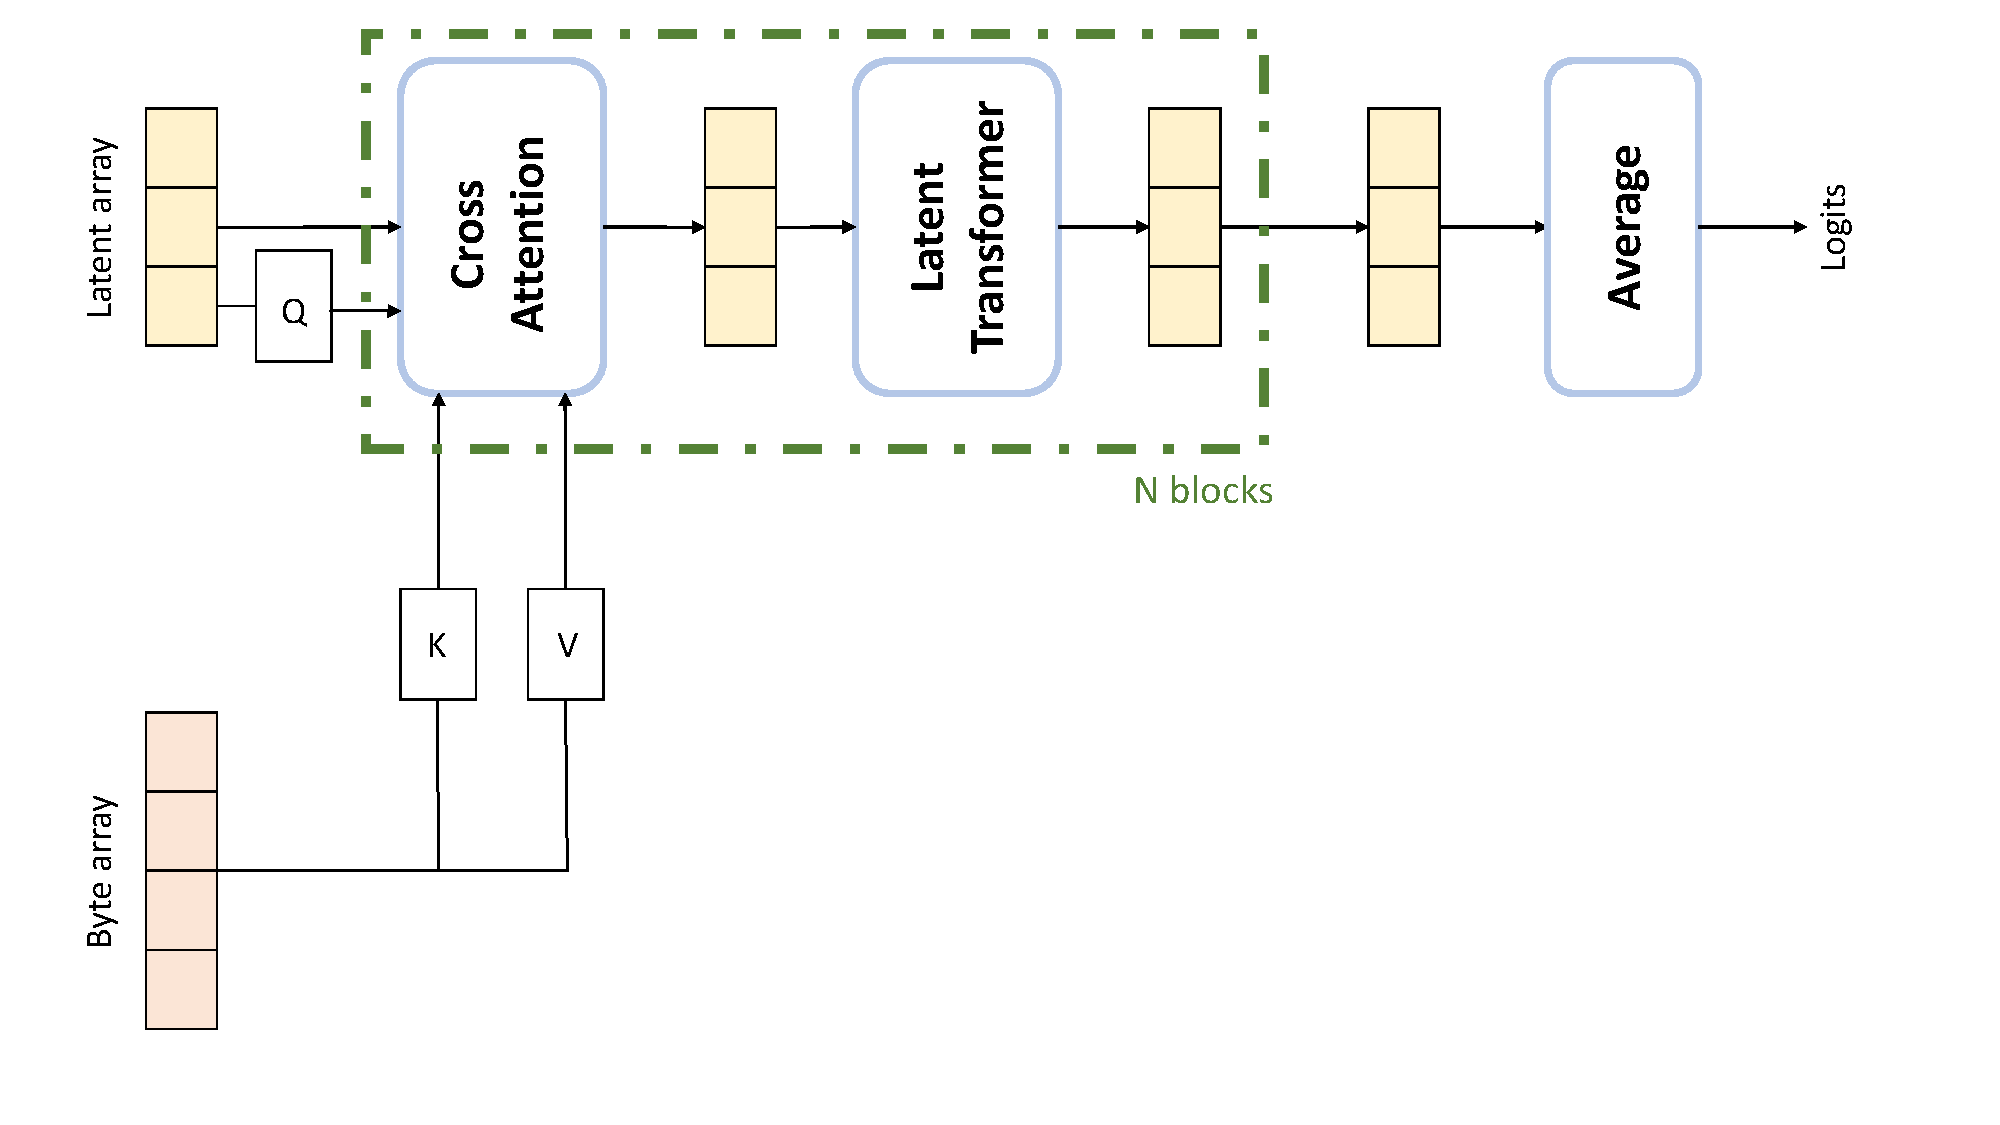
\includegraphics[width=\textwidth,height=\textwidth,keepaspectratio]{images/perceiver.pdf}
  \caption{The perceiver architecture.}
  \label{fig:perceiver}
\end{figure*}

